\documentclass[10pt]{beamer}
\usetheme[
%%% options passed to the outer theme
%    hidetitle,           % hide the (short) title in the sidebar
%    hideauthor,          % hide the (short) author in the sidebar
%    hideinstitute,       % hide the (short) institute in the bottom of the sidebar
%    shownavsym,          % show the navigation symbols
%    width=2cm,           % width of the sidebar (default is 2 cm)
%    hideothersubsections,% hide all subsections but the subsections in the current section
%    hideallsubsections,  % hide all subsections
%    right                % right of left position of sidebar (default is right)
  ]{Aalborg}

\definecolor{aaublue}{RGB}{33,26,82}
\definecolor{aaugrey}{RGB}{84,97,110}

% If you want to change the colors of the various elements in the theme, edit and uncomment the following lines
% Change the bar and sidebar colors:
\setbeamercolor{Aalborg}{fg=aaublue!10,bg=aaugrey!60}
%\setbeamercolor{sidebar}{bg=blue!74}
% Change the color of the structural elements:
\setbeamercolor{structure}{fg=aaublue}
 \setbeamercolor{subtitle}{fg=aaugrey}
% Change the frame title text color:
\setbeamercolor{frametitle}{fg=aaublue}
% Change the normal text color background:
%\setbeamercolor{normal text}{bg=aaugrey!10}
% ... and you can of course change a lot more - see the beamer user manual.
\usebackgroundtemplate{
\includegraphics[width=\paperwidth]{img/background}}

\usepackage[utf8]{inputenc}
\usepackage[english]{babel}
\usepackage[T1]{fontenc}
% ... or whatever. Note that the encoding and the font should match. If T1
% does not look nice, try deleting the line with the fontenc.
\usepackage{lmodern} %optional

% colored hyperlinks
\newcommand{\chref}[2]{%
  \href{#1}{{\usebeamercolor[bg]{Aalborg}#2}}
}

\title[Centralized State Estimation\\ of Distributed Maritime Autonomous Surface Oceanographers]% optional, use only with long paper titles
{Centralized State Estimation of Distributed Maritime Autonomous Surface Oceanographers}

%\subtitle[v.\ 0.1.1] %optional
%{v.\ 0.1.1}

\author[Rasmus L. Christensen, Frederik Juul, Nick \O stergaard, Attila Fodor, Tudor Muresan] % optional, use only with lots of authors
{
  Rasmus L. Christensen, Frederik Juul, Nick \O stergaard, Attila Fodor, Tudor Muresan\\
  {{\tt \{ralch,nickoe,fjuul,afodor12,tmures12\}@es.aau.dk}}
}
% - Give the names in the same order as they appear in the paper.
% - Use the \inst{?} command only if the authors have different
%   affiliation. See the beamer manual for an example

%specify some optional logos
\pgfdeclareimage[height=1.2cm]{mainlogo}{aau_logo.pdf} % placed in the upper left/right corner
\logo{\pgfuseimage{mainlogo}}

\pgfdeclareimage[height=0.75cm]{logo2}{tu-logo} % placed in the lower left/right corner if the \pgfuseimage{logo2} command is uncommented in the \institute command below

\institute[
%  {\pgfuseimage{logo2}}\\ %insert a company or department logo
  Dept.\ of Electronic Systems,\\
  Aalborg University,\\
  Denmark
] % optional - is placed in the bottom of the sidebar on every slide
{%
  Department of Electronic Systems,\\
  Aalborg University,\\
  Denmark
  
  %there must be an empty line above this line - otherwise some unwanted space is added between the university and the country (I do not know why;( )
}
\date{\today}

\begin{document}
% the titlepage
\begin{frame}[plain] % the plain option removes the sidebar and header from the title page
  \titlepage
\end{frame}
%%%%%%%%%%%%%%%%

% TOC
\begin{frame}{Agenda}{}
\tableofcontents
\end{frame}
%%%%%%%%%%%%%%%%
\section{Introduction}
\subsection{Purpose}
% the license
\begin{frame}{Introduction}{Purpose}
  \begin{itemize}
  	\item<1-> Little to no research are currently devoted to maritime autonomous crafts.
    \item<2-> During the 2012 Fukushima accident in Japan, no measurements of the spread of radioactivity was available in the coastal zones, thus relying only on estimates. 
    \item<3-> The coastal area around Greenland has no up-to-date baymethric maps available, and with the growing interest in Greenland (both industrially and commercially) this poses a threat to the ships going in and out of the fjords.
  \end{itemize}
\end{frame}
%%%%%%%%%%%%%%%%

\section{Path planning}
% general installation instructions
\begin{frame}{Path Planning}{Considerations and Description}
    \begin{block}{Considerations}
    \begin{itemize}
    	\item The path planner must be memory efficient.
    	\item The path planner should consider the coastal line to be covered.
    	\item The path planner should create an efficient path.
    \end{itemize}
    \end{block}
    \begin{block}{Straight and Turning segments}
    \begin{itemize}
    	\item Straight segments are generated by having a fixed minimum distance from the shore line, and then define a distance between the measuring lines. This cannot be optimized, as straight lines are, well straight lines. 
    	\item Turning segments are however more interesting, as these can be optimized.
    \end{itemize}
    \end{block}
\end{frame}

% general installation instructions
\begin{frame}{Path Planning}{Theory}
  \begin{block}{Theory}
  \begin{itemize}
     \item<1-> The path planner is based around the Train transition problem, originally solved by. INSERT REF!
    \item<2-> The problem describes that a vehicle in motion, can maintain a linear angular acceleration if the amount of jerk $j$ experienced by the ship is kept constant.
    \item<3-> To keep the jerk $j$ constant, the theory defines the path using the two normalized Fresnel integrals, that when plotted produces the Euler spiral. The Fresnel integrals are given as:
    \begin{align}
    C_F(x) = \int_0^x \cos(t^2)dt,\,\,\,\,S_F(x) = \int_0^x \sin(t^2)dt
\label{eq:fresnel}
    \end{align}
  \end{itemize}
  \end{block}
\end{frame}

% installation on GNU/Linux
\begin{frame}{Path Planning}{Threshold definition}
    \begin{itemize}
    	\item The path planner is also based on the curvature of the turn the ship is to make $\kappa$. This defines if the path should consist of a transition onto a circle, or two Euler spirals (dependent on the curvature).
    	\item The threshold $\varepsilon_\text{max}$ is defined to be:
    	\begin{align}
    	\varepsilon_\text{max} = \frac{\kappa_\text{max}^2}{2 \cdot \eta}
    	\end{align}
    	\item Where $\eta$ is a function described by the highest amount acceleration the ship can experience and the velocity at which it traverses this.
    	\begin{align}
    	\eta = \frac{\alpha_\text{max}}{v^2_\text{max}}
    	\end{align}
    	\item This function allows the ship to preserve as much energy as possible, without veering out of course.
    \end{itemize}
\end{frame}
%%%%%%%%%%%%%%%%

\subsection{Waypoint generation}
% installation on GNU/Linux
\begin{frame}{Path Planning}{3-point scenario}
    \begin{itemize}
    \item The below figure shows the waypoints generated by the ship when $\varepsilon < \varepsilon_\text{max}$. This consists of an inward and an outward Euler spiral. 
    	\begin{figure}
			\begin{center}
				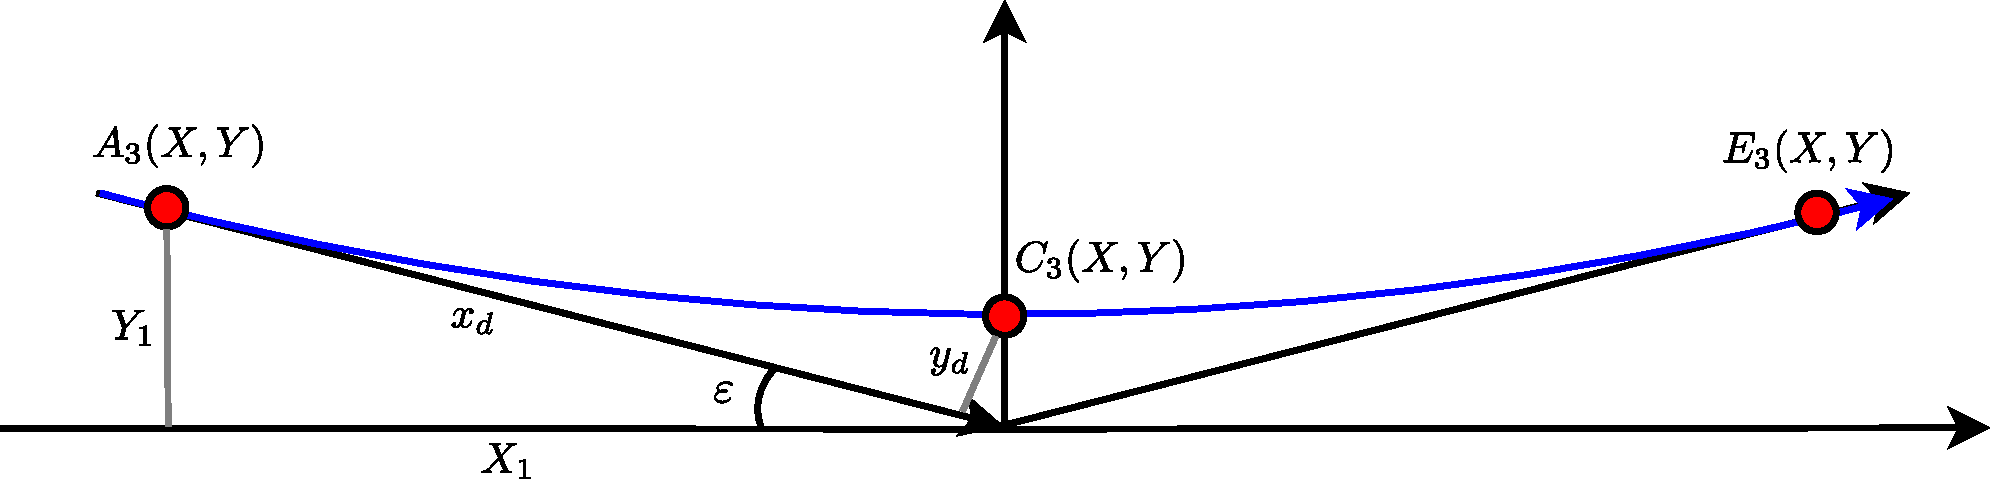
\includegraphics[width=8.4cm]{img/3Points} % width of a column is 8.4 cm.
				\label{fig:3points}
			\end{center}
		\end{figure}
		\item The waypoints are computed as follows:
		\begin{align}
		A_3 = (-X_1,Y_1),\, C_3 = (0,\frac{y_d}{\cos(\varepsilon)}),\, E_3 = (X_1,Y_1)
		\end{align}
		\item Where $X_1$ and $Y_1$ can be computed as functions of the normalized Euler spirals, with $x_d$ and $y_d$ representing the length:
		\begin{align}
X_1 = x_d \cdot \cos(\varepsilon) + y_d \cdot \sin(\varepsilon),\,\, Y_1 = X_1 \cdot \tan(\varepsilon)
		\end{align}
    \end{itemize}
\end{frame}
%%%%%%%%%%%%%%%%

% installation on GNU/Linux
\begin{frame}{Path Planning}{5-point scenario}
    \begin{itemize}
    \item The below figure shows the waypoints generated by the ship when $\varepsilon > \varepsilon_\text{max}$. This consists of a transition from an inward Euler spiral, onto a circle and then a transition from the circle onto an outward Euler spiral. 
    	\begin{figure}
			\begin{center}
				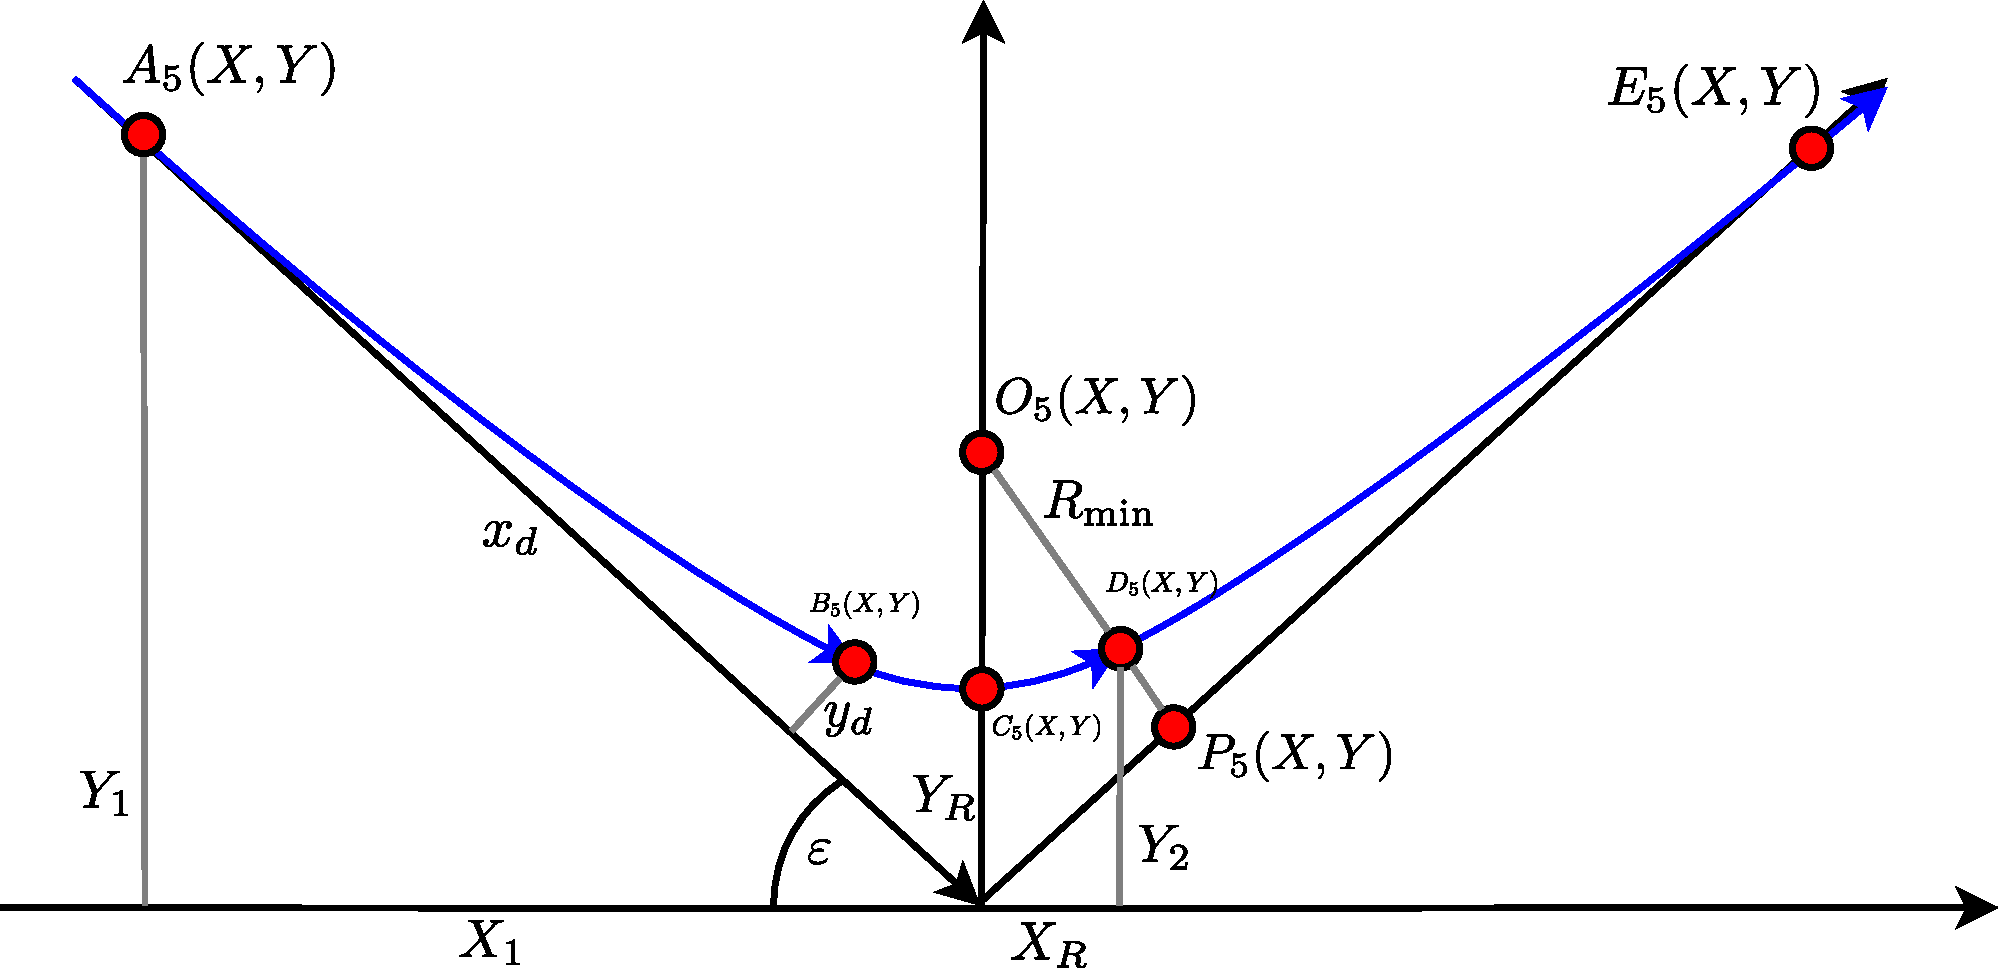
\includegraphics[width=8.4cm]{img/5Points}
				\label{fig:5points}
			\end{center}
		\end{figure}
		\item Adding the two points $B_5$ and $D_5$ given as:
		\begin{align}
		B_5 &= (-R_\text{min} \cdot \sin(\varepsilon - \varepsilon _\text{max}),\,\, Y_1 - x_d \cdot \sin(\varepsilon))\\
		D_5 &= (R_\text{min} \cdot \sin(\varepsilon - \varepsilon _\text{max}),\,\, Y_1 - x_d \cdot \sin(\varepsilon))
		\end{align}
    \end{itemize}
\end{frame}
%%%%%%%%%%%%%%%%

\subsection{Verification}
% installation on Microsoft Windows
\begin{frame}{Path Planning}{Verification}
  \begin{itemize}
  	\item To verify that the planner works properly, a random shoreline have been generated using a random walk, and a bounding box was drawn, the algorithm was then programmed to generate a shoreline, producing the following results:
  	\begin{figure}
			\begin{center}
				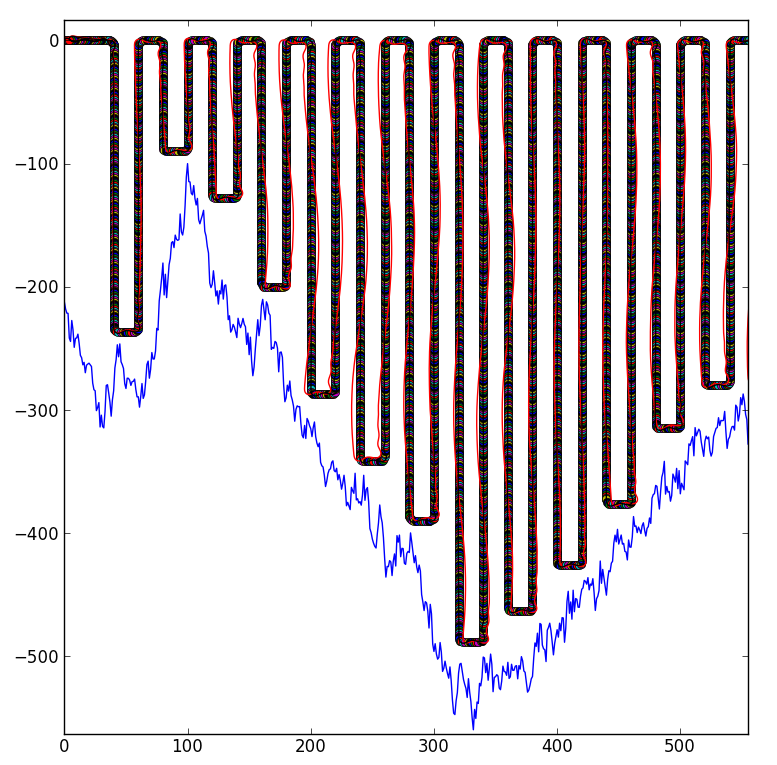
\includegraphics[width=5cm]{img/Auto_WP_Planning}
				\label{fig:5points}
			\end{center}
		\end{figure}
		\item The dots on the figure represent the waypoints.
  \end{itemize}
\end{frame}
%%%%%%%%%%%%%%

\section{Modeling and Control}
\begin{frame}{Modeling and Control}{Consideration and Description}
  \begin{block}{Considerations}
    The model is built using a top-down approach, running the main controls on a high-level interface (HLI). A low-level interface (LLI) handles the actuators and reads all the sensors. The link between these are a simplex 19.2 kbps radio link.
  \end{block}
  \begin{block}{Top layer - HLI}
    Receives the sensor readings from the LLI and computes actuator set-points which are transmitted to the LLI. 
  \end{block}
  \begin{block}{Bottom layer - LLI}
  Receives the actuator set-points and sets these, then reads the sensors and transmit these readings back. 
  \end{block}
\end{frame}
%%%%%%%%%%%%%%%%

% list of the themes and options
\subsection{Theory}
\begin{frame}{Modeling and Control}{State space representation}
  \begin{block}{Assumptions}
    The model is simplified to a 3-DOF model, with only motion in the $x$ and $y$ direction, as wel as rotation about the $z$-axis defined as $\theta$. The model does not take into account the surge generated by the ship as it moves in the water, and the effects of planing is not taken into account, as the ship is not moving faster than $\approx$ 1 m/s.
    With these assumptions the following contiuous time state space model have been derived:
  \begin{align}
  \dot{\begin{bmatrix}
v\\
\theta\\
\omega
\end{bmatrix}} = \begin{bmatrix}
-\beta_v & 0 & 0\\
0 & 0 & 1\\
0 & 0 & -\beta_\omega
\end{bmatrix} \begin{bmatrix}
v\\
\theta\\
\omega
\end{bmatrix} + \begin{bmatrix}
m^{-1} & 0\\
0 & 0\\
0 & I^{-1}
\end{bmatrix}\begin{bmatrix}
F\\
\tau
\end{bmatrix}
  \end{align}
    \end{block}
    4 non-linear terms appear in the equation. Namely the $\beta$ terms and the computations of the forward force $F$ and the torque $\tau$.
\end{frame}
%%%%%%%%%%%%%%%%

\begin{frame}{Modeling and Control}{Linearization}
  \begin{block}{$F$ and $\tau$ terms}
  The force $F$ and torque $\tau$ are dependent on the same variables, namely the number of revolutions of the propellers $n_1$ and $n_2$. These can be computed by:
  \begin{align}
\begin{bmatrix}
n_1^2\\
n_2^2
\end{bmatrix} = \begin{bmatrix}
C_1 & C_1\\
C_1 \cdot l \cdot \sin(\theta_\text{stbd.}) & C_1 \cdot l \cdot \sin(\theta_\text{port})
\end{bmatrix}^{-1}\begin{bmatrix}
F_\text{desired}\\
\tau_\text{desired}
\end{bmatrix}\label{eq:solver}
\end{align}
Solving for $n_1$ and $n_2$ produces:
\begin{align}
n_1 = \frac{n_1^2}{\text{abs}\{n_1^2\}} \cdot \sqrt{n_1^2},\,\, n_2 = \frac{n_2^2}{\text{abs}\{n_2^2\}} \cdot \sqrt{n_2^2}
\end{align}
  \end{block}
  \begin{block}{$\beta$ term}
  The $\beta$ terms are linearized using a Taylor approximation. The constant term is removed in the reference gain of the controller.
  \end{block}
\end{frame}
%%%%%%%%%%%%%%%%

\begin{frame}{Modeling and Control}{Controllers}
\begin{block}{Optimal feedback gain and reference tracking}
The optimal state feedback gain is computed by minimizing the cost function $\mathcal{J}$, given as:
\begin{align}
\mathcal{J} = \int_0^\infty (x^T(t)\cdot Q\cdot x(t) + u^T(t) \cdot R \cdot u(t))dt
\end{align}
Producing the following feedback gain:
\begin{align}
F_\text{opt} = \begin{bmatrix}
15.1668 & 0 & 0\\
0 & 2.5165 & 0.7134
\end{bmatrix}
\end{align}
\end{block}
The reference gain is computed by augmenting the system as in INSERT REF!, thus producing the reference gain:
\begin{align}
N_\text{reference} = \begin{bmatrix}
24.0668 & 0\\
0 & 2.5165 \end{bmatrix}
\end{align}
\end{frame}

\subsection{Verification}
\begin{frame}{Modeling and Control}{Verification}
Through simulations, the system have produced the following figures used to verify wether the controller strategy.
  	\begin{figure}
			\begin{center}
				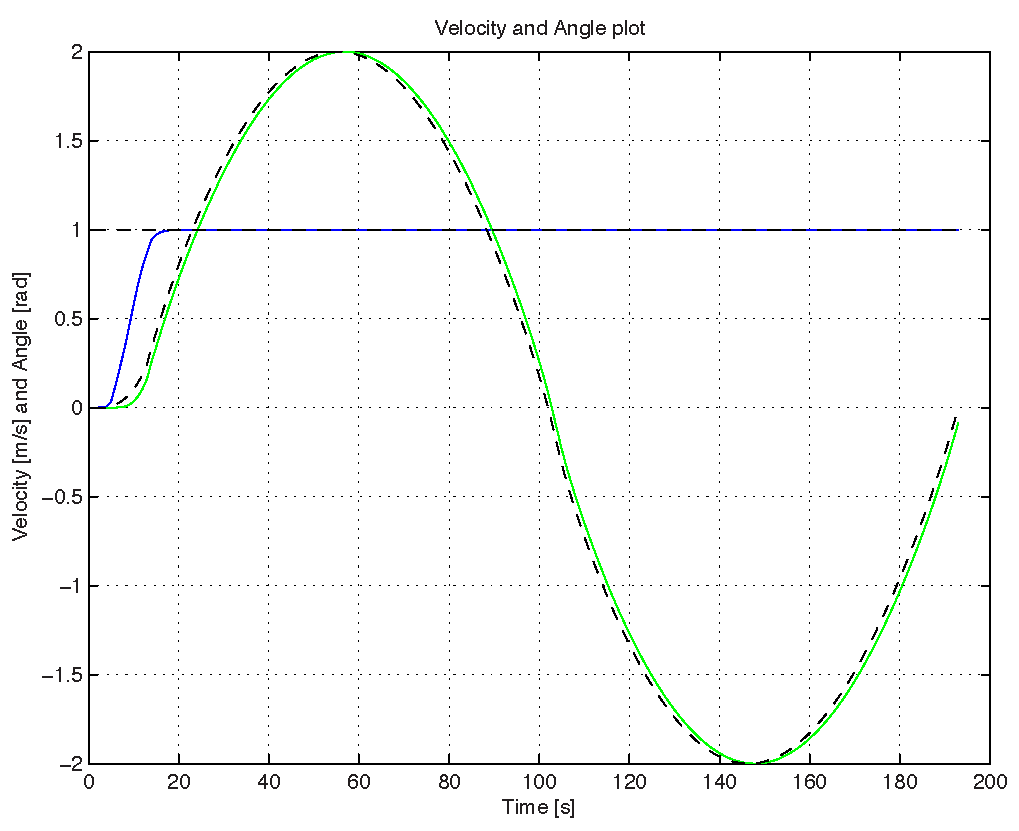
\includegraphics[width=8.2cm]{img/reftrack}
				\label{fig:reftrack}
			\end{center}
		\end{figure}
\end{frame}
%%%%%%%%%%%%%%%%

\begin{frame}{Modeling and Control}{Verification}
And testing if the conversion from desired force to revolutions work. 
  	\begin{figure}
			\begin{center}
				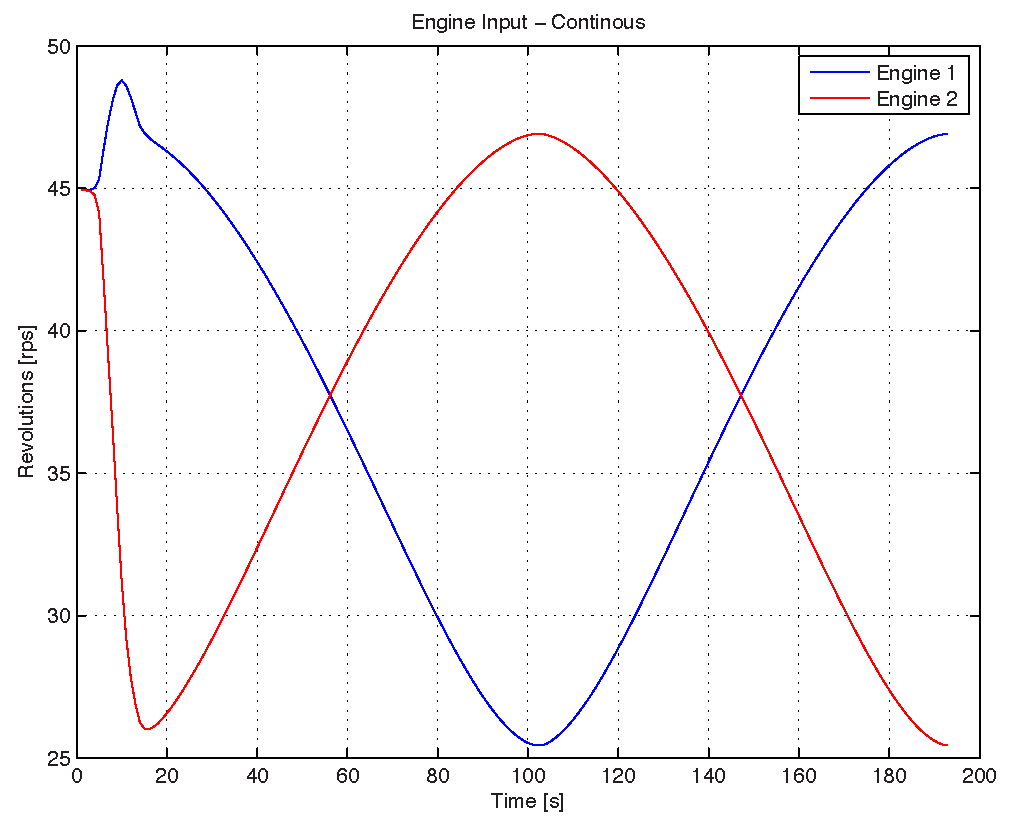
\includegraphics[width=8.2cm]{img/eng_inp}
				\label{fig:eng_inp}
			\end{center}
		\end{figure}
\end{frame}

%%%%%%%%%%%%%%%%%%

\section{State estimation}
\subsection{Theory}
% help me iron out the bugs or give me some comment and suggestions
\begin{frame}{State Estimation}{Theory}
\begin{block}{Estimated states and input state model}
The estimated states are defined as:
\begin{align}
^b\hat{x_k} = \begin{bmatrix}
x & \dot{x} & y & \dot{y} & \theta & \omega
\end{bmatrix}^T
\end{align}
As the ship is fitted with an IMU and a GPS, the measured states becomes:
\begin{align}
v_k = \begin{bmatrix}
x & \dot{x} & \ddot{x} & y & \dot{y} & \ddot{y} & \theta & \omega & \alpha
\end{bmatrix}^T
\end{align}
Giving the state model of the system as (ts = 20 Hz):
\begin{align}
\Phi = diag\{\Phi _x,\Phi _y,\Phi _\omega\}
\end{align}
Where the individual $\Phi$s are given as:
\begin{align}
\Phi_{x,y,\omega}(k) = \begin{bmatrix}
1 & t_s & 0\\
0 & 1 & t_s\\
0 & -\beta_{x,y,\omega} & 0
\end{bmatrix}
\label{eq:kal}
\end{align}
\end{block}
\end{frame}

\begin{frame}{State Estimation}{Theory - zero gaining}
As the LLI and HLI are run on two seperate computers, the Kalman filter needs to filter out the measurements which are invalid. This is done by multiplying the Kalman gain $\bar{K}$ by a validity mask-matrix $\Lambda$, given as:
\begin{align}
\Lambda = diag\{ \lambda_x,\lambda_{\dot{x}},\lambda_{\ddot{x}},\lambda_y,\lambda_{\dot{y}},\lambda_{\ddot{y}},\lambda_{\theta},\lambda_{\omega},\lambda_{\alpha} \}
\end{align}
Where the $\lambda$s are defined as:
\begin{align}
\lambda = 
\left\{
  \begin{array}{l l}
    1 & \quad \text{if checksum is valid}\\
    0 & \quad \text{otherwise}
  \end{array} \right.
\end{align}
\end{frame}

\subsection{Verification}
\begin{frame}{State Estimation}{Verification of State estimator}
A test of the Kalman filter, to see if it estimates lost packages was carried out producing. Figure (b) represents the case where GPS measurements are lost for 60 seconds:
\begin{figure}
			\begin{center}
				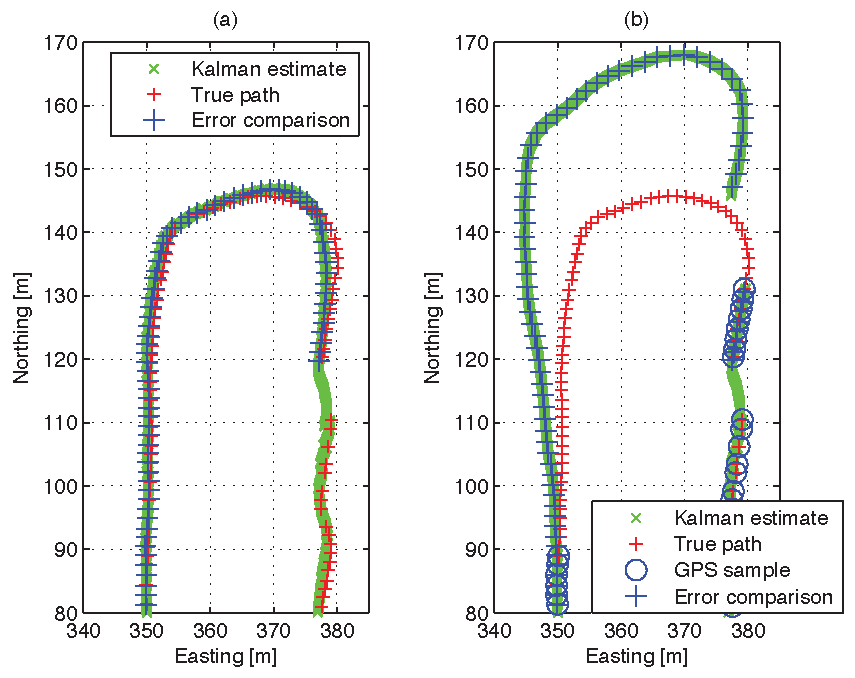
\includegraphics[width=8.2cm]{img/track}
				\label{fig:track}
			\end{center}
		\end{figure}
\end{frame}

\begin{frame}{State Estimation}{Verification of State estimator}
The absolute error of the position are depicted on the figure below:
\begin{figure}
			\begin{center}
				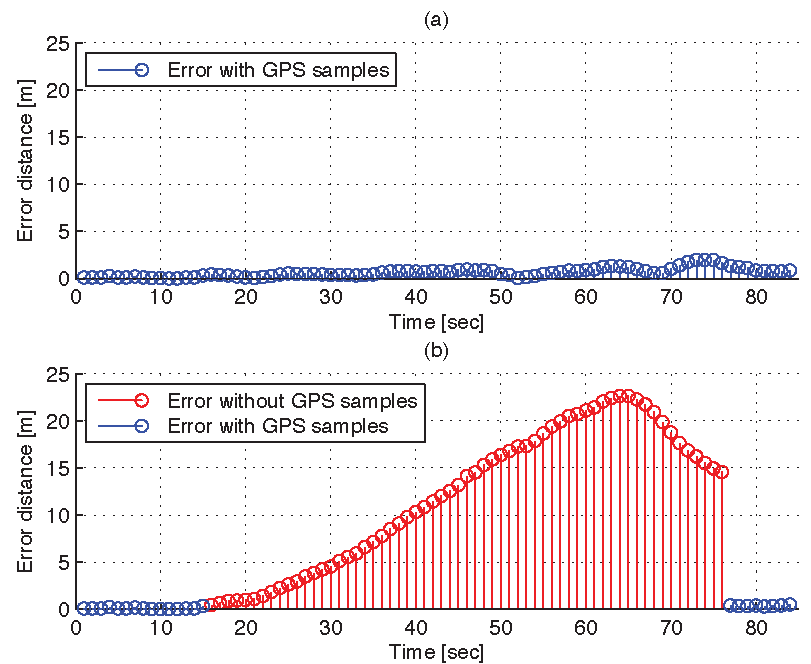
\includegraphics[width=8.2cm]{img/error}
				\label{fig:error}
			\end{center}
		\end{figure}
\end{frame}
%%%%%%%%%%%%%%%%

\section{Final test}
\subsection{Kalman estimator}
\begin{frame}{Final test}{Kalman estimator verification}
As the waters around Aalborg have frozen solid, final tests in water have not been carried out, however, tests on land have been carried out, producing the following:
\begin{figure}
			\begin{center}
				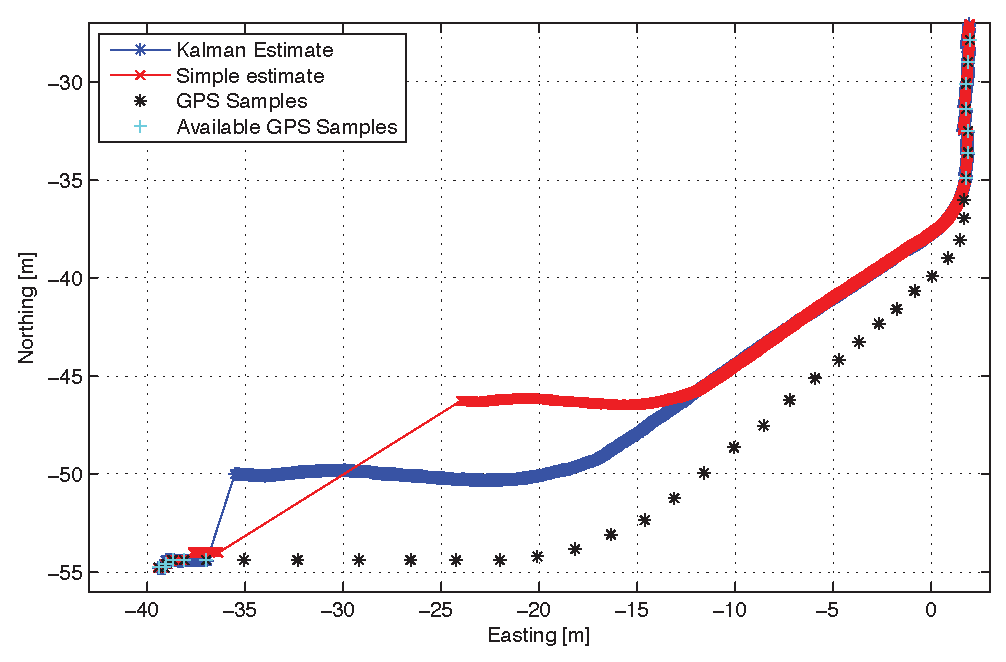
\includegraphics[width=8.2cm]{img/kalmanestimate}
				\label{fig:kalmanestimate}
			\end{center}
		\end{figure}
\end{frame}

\subsection{Controller}
\begin{frame}{Final test}{Engine input verification}
Producing the engine inputs from the controller.
\begin{figure}
			\begin{center}
				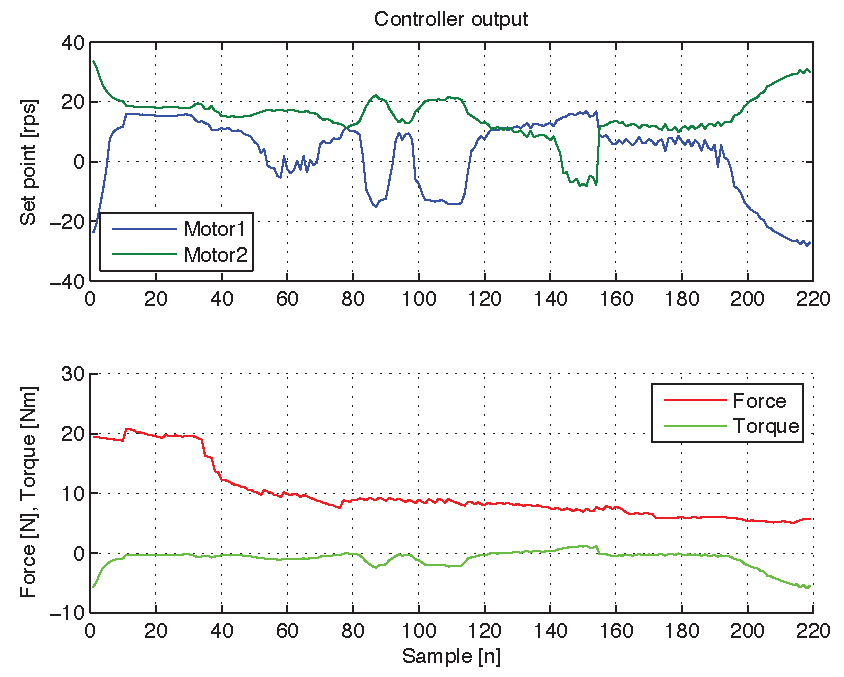
\includegraphics[width=8.2cm]{img/motorinput}
				\label{fig:motorinput}
			\end{center}
		\end{figure}
\end{frame}
%%%%%%%%%%%%%%%%

\end{document}
